\chapter{Objetivos}\label{cap.objetivos}
En este punto ya hemos introducido el contexto en el que desarrolla el trabajo, de manera que es momento de describir los objetivos que se han tratado de alcanzar, los requisitos para ellos y la metodología a seguir para su consecución.

\section{Objetivos}
La meta de este proyecto consiste en la creación de 2 nuevas prácticas para el entorno docente JdeRobot-Academy desde el principio, incluyendo todas las comunicaciones correspondientes, el nodo académico, la interfaz gráfica y el código auxiliar, los modelos e incluso una solución de referencia al ejercicio. Así, en cada una de las nuevas prácticas, que consistirán en seguimiento de caras a través de una cámara y auto localización basada en láser, se elaborará toda la infraestructura que se comunica con el Simulador Gazebo, donde el alumno podrá ver el resultado de la ejecución de su algoritmo. Se ofrecerá, en cada práctica, un fichero MyAlgorithm.py donde el alumno programará su solución.

Cabe entrar un poco más en detalle acerca de lo que se pretende con cada práctica creada:
\vspace{0.6cm}

En primer lugar, la práctica de seguimiento de caras, a la que a partir de ahora nos referiremos como \textbf{Follow Face}, busca que el alumno adquiera o ponga en práctica sus conocimientos de segmentación de imagen, a través de la cual buscará en la imágenes que le sirve una cámara hardware posibles caras de personas, obtendrá datos de posición de las mismas y los transformará en órdenes para la cámara que no son más que movimientos en el eje horizontal y vertical, más conocidos como \textit{Pan} y textit{Tilt} respectivamente.

La segunda práctica creada es la de auto localización basada en láser o \textbf{Laser} Loc, donde se trata de que el alumno programe un algoritmo de auto localización a través del método no determinista de Montecarlo del filtro de partículas, de tal manera que se teleoperará un robot de la marca iRobot modelo \textit{Create} (versión americana del robot \textit{Roomba}) que deberá saber en todo momento en qué lugar del escenario se encuentra, acercándonos a su vez a sistemas robóticos que ya existen en el mercado y con ello aprender cómo funcionan.
\vspace{0.6cm}

Con todo ello, en este proyecto se tratará de:
\vspace{0.5cm}

\begin{itemize}%[leftmargin=1em]
  \renewcommand{\labelitemi}{$\to$}
 \item Realizar un trabajo previo de aprendizaje de la infraestructura de JdeRobot y pulimentar las prácticas existentes.
  \item Asentar las bases de la simulación de robots, creando modelos y escenarios móviles e interactivos.
  \item Aprender las formas de comunicación entre robots y middleware.
  \item Crear las dos nuevas prácticas mencionadas.
  \item Programar soluciones de referencia para las prácticas, en cuyo camino se obtendrá conocimiento del funcionamiento de los robots.
	\item Estudiar nuevas tecnologías en el camino hacia una aplicación multiplataforma, IPython 3.0.
	\item Añadir versatilidad a través de ROS, acercándonos a la estructura empleada por robots reales.
	\item Obtener conclusiones acerca de lo estudiado, con las cuáles completar la formación en el campo.
\end{itemize}

\section{Requisitos previos} 
El desarrollo del proyecto se ha basado en subdividir las metas en pequeños subobjetivos que juntos compondrán los propósitos mencionados anteriormente, siempre supeditado a los requisitos de partida del proyecto, los cuales hacen que la solución esté condicionada:

\begin{enumerate}
	\item Todas las simulaciones se realizarán en el simulador Gazebo, en concreto en la versión 7.9.0. Los modelos de robots que se emplearán serán creados. En este caso se utilizará el robot \textit{Create} modificado con un sensor láser. En cuanto a los modelos del mundo de Gazebo, habrá que estudiar las distintas opciones.
	\item Se hará uso del middleware robótico JdeRobot en su versión 5.6.1 desarrollada recientemente, que se explicará con detalle en el Capítulo 3. El uso de esta plataforma simplifica el desarrollo del comportamiento del robot.
	\item El sistema operativo que se empleará para este proyecto será Ubuntu 16.04 LTS.
	\item El lenguaje de desarrollo empleado para crear los distintos componentes será Python, en concreto en su versión 2.7.12. Por compatibilidad con JdeRobot-5.6.1 y de éste con el middleware ROS \textit{Kinetic} no se ha usado Python-3.x
	\item Las soluciones han de ejecutar algoritmos que funcionen en tiempo real, de manera que deberán ser eficientes y ejecutar movimientos suaves para no estropear el hardware si lo hay.
\end{enumerate}

\section{Metodología}
La elaboración de este trabajo podría descomponerse en un conjunto de iteraciones con varias fases, en cada una de las cuales se establecía una reunión con el tutor para determinar los subobjetivos, planificar como abordarlos, analizar los posibles problemas y corregir fallos. Así, se ha conseguido un desarrollo fluido y completo, asentando los conocimientos y despejando las dudas que surgían a lo largo de los meses que se dedicó al trabajo.

Parte del seguimiento lo hemos hecho utilizando herramientas de apoyo, como la bitácora semanal en la Wiki de JdeRobot \footnote{\url{https://jderobot.org/Cawadallah-tfg}} donde periódicamente se redactaban los avances realizados y se añadían vídeos demostrativos de lo conseguido, imágenes representativas y texto descriptivo. El código asociado a los avances se almacenó en un repositorio personal de GitHub\footnote{\url{https://github.com/cawadall/Academy}}\footnote{\url{https://github.com/cawadall/JdeRobot}}, al que el tutor ha podido acceder en todo momento para aportar \textit{feedback} y favorecer el progreso.

Así las cosas, se ha optado por seguir el modelo de desarrollo en espiral creado por Barry Boehm, el cual hemos creído que se adaptaba perfectamente a nuestras necesidades, permitiéndonos separar el comportamiento final en varias sub-tareas más sencillas, a la par que disponer de flexibilidad ante cambios en los requisitos, algo bastante común a medida que avanzaba el desarrollo. Con él, conseguimos una resolución temprana de riesgos y poder definir la arquitectura en las fases iniciales, todo ello basado en un proceso continuo de verificación de la calidad.

\begin{figure}[H]
  \begin{center}
    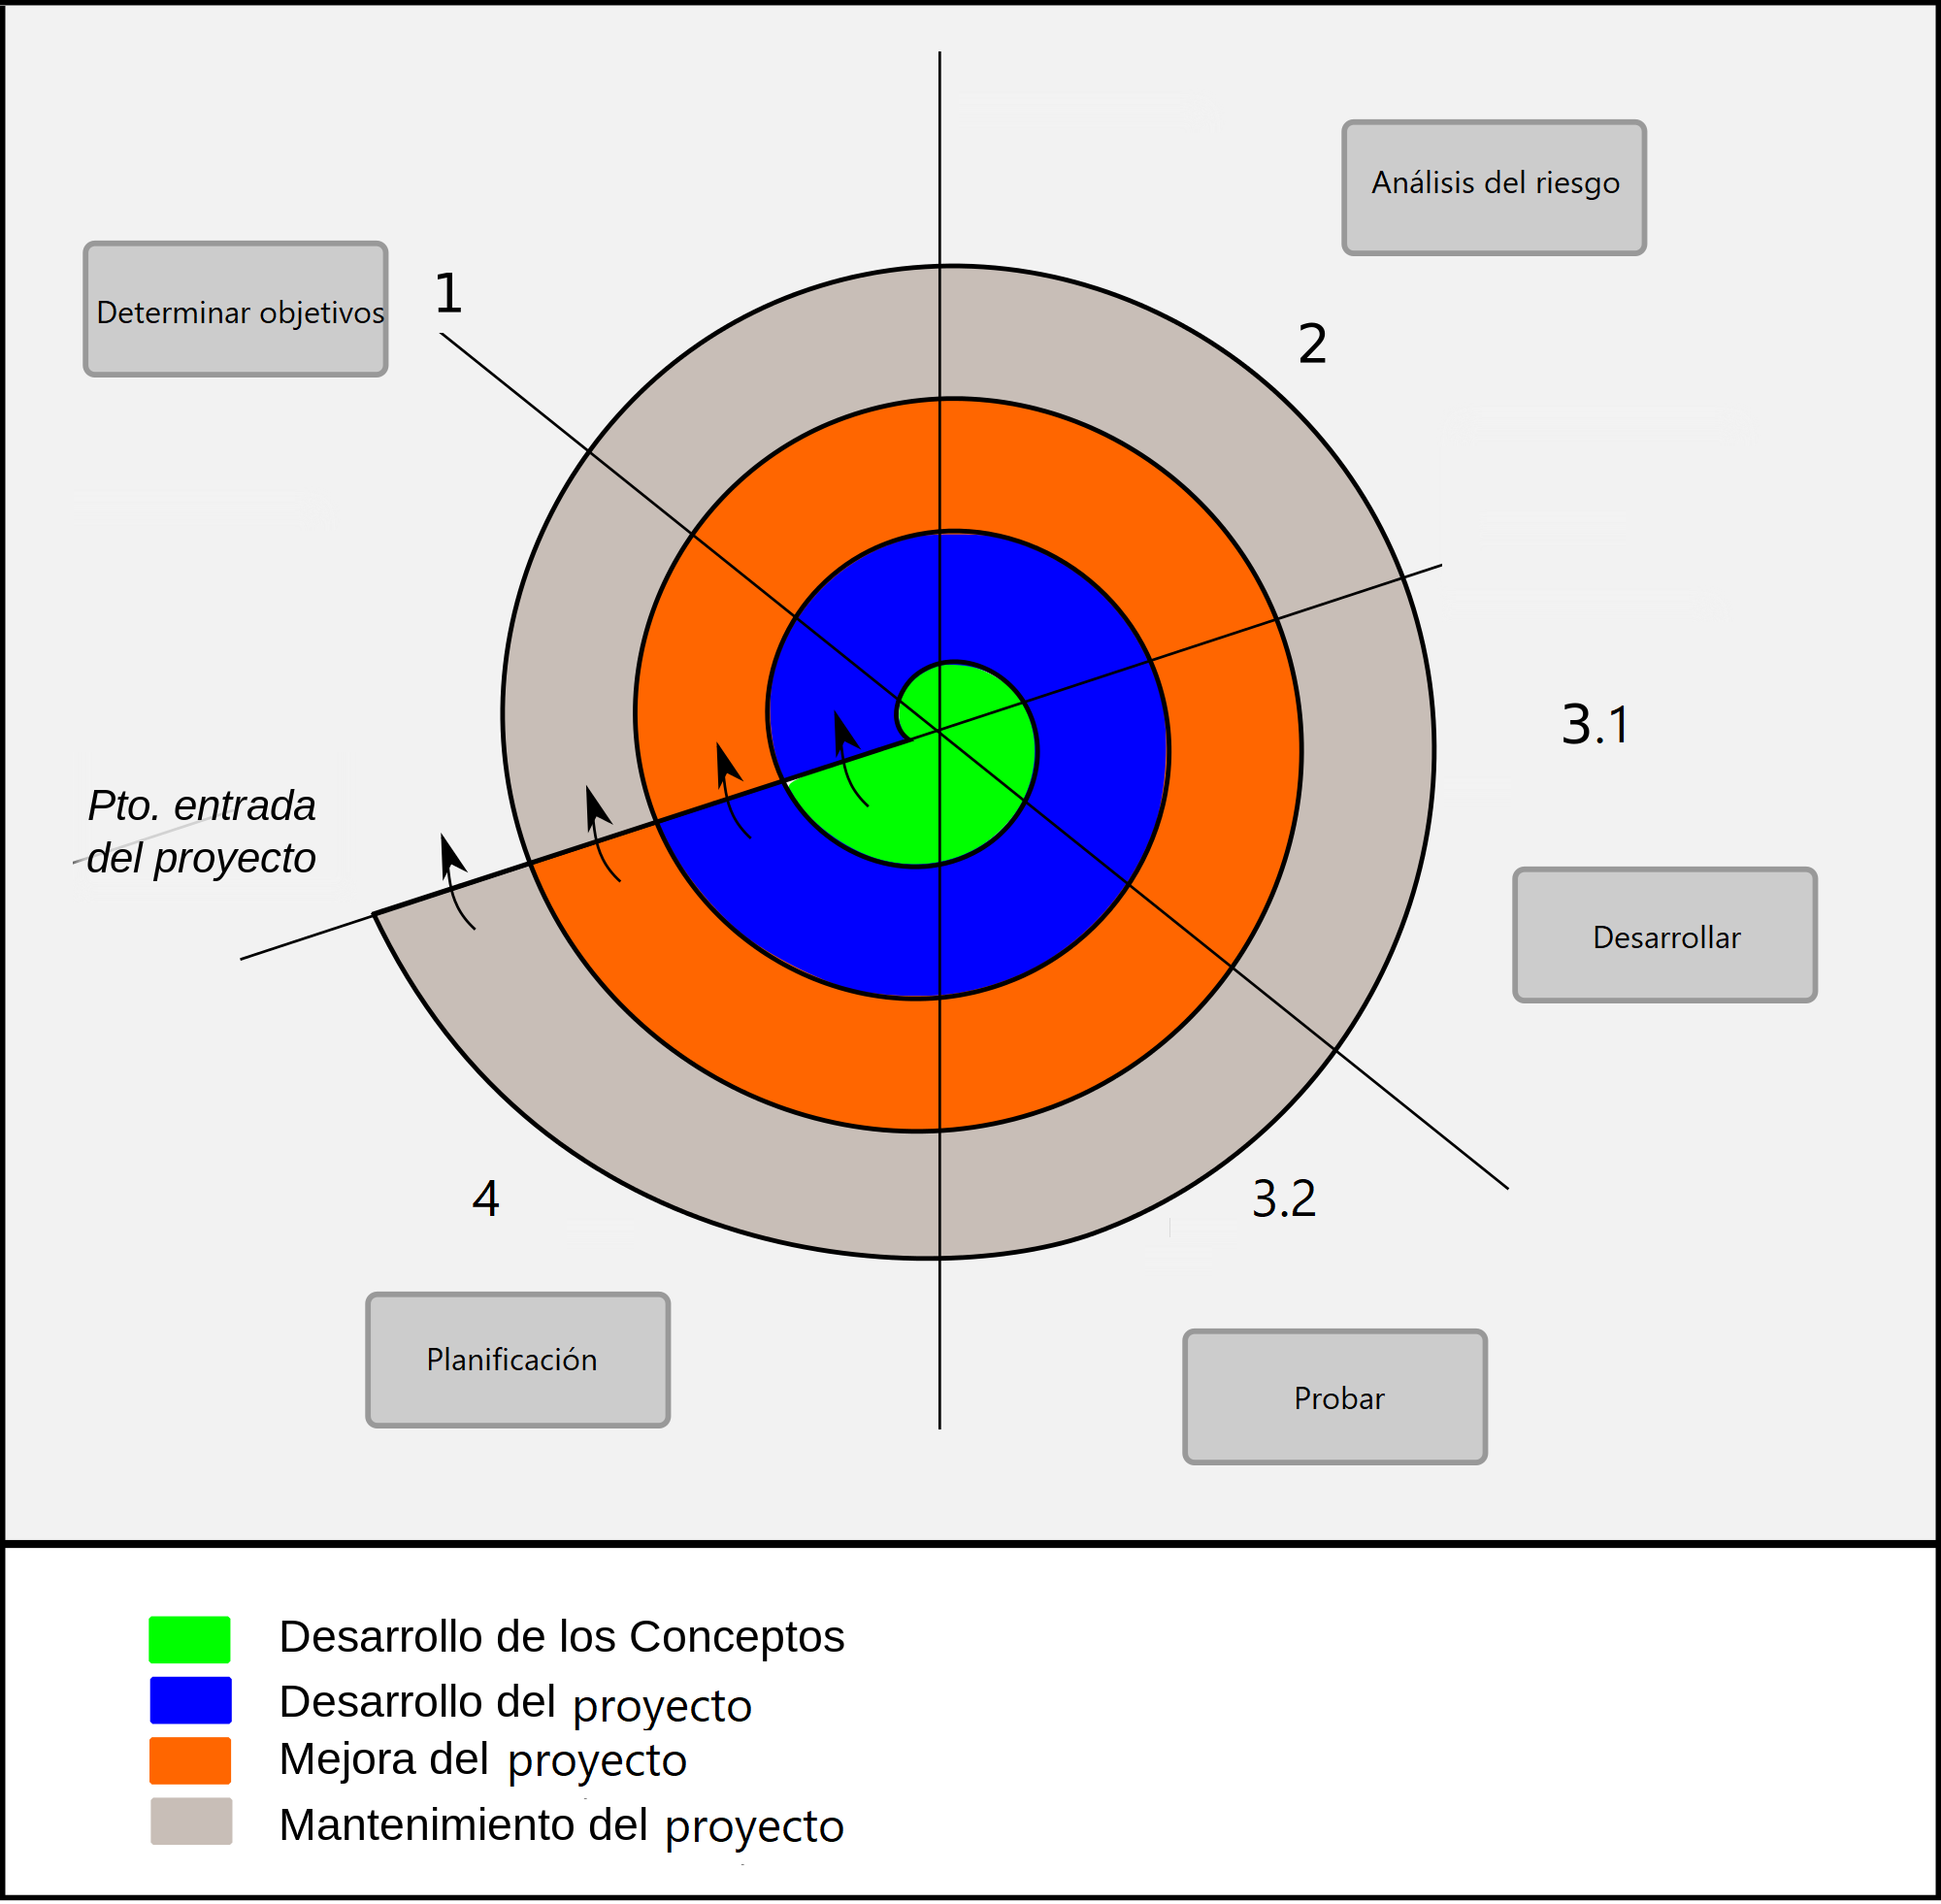
\includegraphics[width=0.9\linewidth]{figures/modelo_espiral.png}
		\caption{Modelo de desarrollo en espiral}
		\label{fig.espiral}
		\end{center}
\end{figure}

Como se puede ver en la \textbf{Figura 2.1}, este modelo de ciclo de vida permite ir obteniendo prototipos funcionales en primera instancia, luego mejorar el prototipo conseguido y, por último, pulir los detalles para cubrir todos los requisitos.  Así, se realiza el trabajo de forma incremental, en forma de ciclos con cuatro fases bien definidas:

\begin{itemize}
	\item[--] \textbf{Determinar objetivos}: en esta primera fase del ciclo se definen los objetivos que se deben de llevar a cabo para que una vez completados se pueda dar por finalizado el mismo.
	\item[--] \textbf{Análisis del riesgo}: en la segunda fase se evalúa qué problemas es posible encontrarse al empezar el desarrollo, y pensar en cómo abordarlos.
	\item[--] \textbf{Desarrollar y probar}: ya en la tercera fase es en la que, tras evaluar los riesgos, se procede al propio desarrollo del trabajo, además de las correspondientes pruebas para verificar su correcta funcionalidad.
	\item[--] \textbf{Planificación}: en esta última fase se valoran los resultados obtenidos en el ciclo y se planifican las siguientes etapas del proyecto.
\end{itemize}

Una vez establecida la metodología del trabajo, es hora de ponerla en práctica para llevar a cabo la parte práctica del proyecto.

\section{Plan de trabajo}
Para lograr los objetivos ya descritos, se han seguido las siguientes etapas:

\begin{itemize}
	\item[--] \textbf{Familiarización con el entorno JdeRobot}. Tras la descarga e instalación del software  involucrado, incluyendo dependencias, simulador y bibliotecas necesarias, se tratará de entrar en contacto con el entorno JdeRobot modificando las prácticas existentes para añadir mejoras en sus interfaces gráficas, llevar a cabo una actualización de todas ellas para que funcionen con la nueva biblioteca de comunicaciones JdeRobotComm incluida en esta nueva versión 5.6.X, e incluso programar la solución para algunas de las prácticas.
	\item[--] \textbf{Toma de contacto con el simulador Gazebo}. En esta etapa se han estudiado distintos ejemplos disponibles en la web de Gazebo\footnote{\url{http://gazebosim.org/tutorials}} y de JdeRobot. Además, se ha estudiado el funcionamiento básico de los \textit{plugins}  que Gazebo emplea para controlar los robots, sus sensores y sus actuadores. Esto ha implicado la investigación del lenguaje de programación C++, el cual también ayudará a comprender la migración de las comunicaciones a \textit{plugins} ROS.
	\item[--] \textbf{Estudiar las bibliotecas involucradas}, entre las cuales destacan OpenCV, Threading, NumPy y PyQt5.
\end{itemize}

Una vez aquí, para cada práctica…

\begin{itemize}
	\item[--] \textbf{Crear los mundos y modelos necesarios y puesta a punto del hardware}.  Se ha empleado distintos \textit{plugins} para la simulación d ella funcionalidad del robot, se ha creado distintos mundos para realizar pruebas, y se ha construido un driver para poder manejar el hardware, en el que entraremos más adelante.
	\item[--] \textbf{Desarrollar la infraestructura}, que consta la interfaz gráfica, el nodo de comunicaciones, el fichero plantilla y el código auxiliar.
	\item[--] \textbf{Realizar las soluciones}, construyendo un algoritmo para ambas prácticas.
	\item[--] \textbf{Extrapolar la solución y el nodo a IPython}, herramienta explicada en el apartado 3.6.
	\item[--] \textbf{Adaptar las prácticas a ROS}, ya que en principio se establecerán las comunicaciones con ICE. 
\end{itemize}